\documentclass[11pt]{article}
\usepackage[a4paper,margin=20mm,top=18mm,bottom=18mm]{geometry}
\usepackage[T1]{fontenc}
\usepackage[utf8]{inputenc}
\usepackage{lmodern,graphicx,amsmath,microtype,xcolor}
\usepackage[colorlinks=true,urlcolor=teal]{hyperref}
\setlength{\parindent}{0pt}
\setlength{\parskip}{6pt}
\definecolor{deep}{HTML}{173A47}
\newcommand{\heading}[1]{\par\vspace{5pt}{\Large\bfseries\color{deep}#1}\par}
\begin{document}
{\Huge\bfseries Writing pictured facts into Chinese sentences\par}
{\large Imagized Language Model research report}\par
\heading{Abstract}
A model can write both the correct price and the correct address while assigning the price to the address. We trained a visual reader to locate the properties requested in a human question and a recurrent writer to track the property it is expressing. Both components fitted from scratch on one RTX 4090 D in 27.2 seconds and together contain 333,850 parameters. On 37 held Chinese dialogue turns labelled with two fields, the earlier aligned writer printed clean pairs of values on 36 but explicitly attached each to the appropriate property on only 24. The compact writer passed both tests on 36. It returned a clean value on all 515 eligible single-field turns. Fourteen further turns were admitted after the model was frozen. It passed twelve. The experiments concern one supplied, aligned venue record and eight scalar fields.

\heading{A wrong sentence with two correct values}
A guest asked for the price and address of a hotel. The earlier writer began by saying its address was 1,354 yuan. Its planned evidence was correct. Its choice of words reversed the meaning. The compact writer used the same plan and the same source pixels. This time it said the price was 1,354 yuan and gave the street as the address (Fig.~1). After masking the copied material, the compact writer used nineteen distinct wordings for nineteen distinct domain and ordered-field combinations across the 37 turns. Its repertoire is narrow.

\heading{Where the learning signal enters}
For each visible query position $t$ and candidate field $i$ the reader learns a local score $z_{ti}$. For a pair of fields it combines the evidence for $i$ at one glyph position and $j$ at any later position, summing over all such alignments. A single prefix sum per field computes this quantity. The model can also choose one field. As the writer draws each clause it sees the current field, the preceding field and any remaining field. Copying the current source span advances the plan. Lexical glyphs, connectors and punctuation are learned from human replies. A stop is legal when the plan is complete. One Lean proof establishes the alignment sum. A second characterizes every accepted pointer sequence. Neither proof asserts that a field was read correctly.

\heading{What the comparator tells us}
Matched byte reading passed 37/37 and used 2.51 kJ to fit the complete system, versus 2.58 kJ for the image model. The local Qwen3-8B text comparator scored 35/37 on literal values. One miss was a correct municipal address variant. On the other, it correctly answered three requested facts where the annotations listed two. The compact writer omitted one. \href{https://aclanthology.org/2020.tacl-1.19/}{CrossWOZ dialogue source}.
\newpage
\heading{Figure 1. Which fact does this clause express?}
\begin{center}
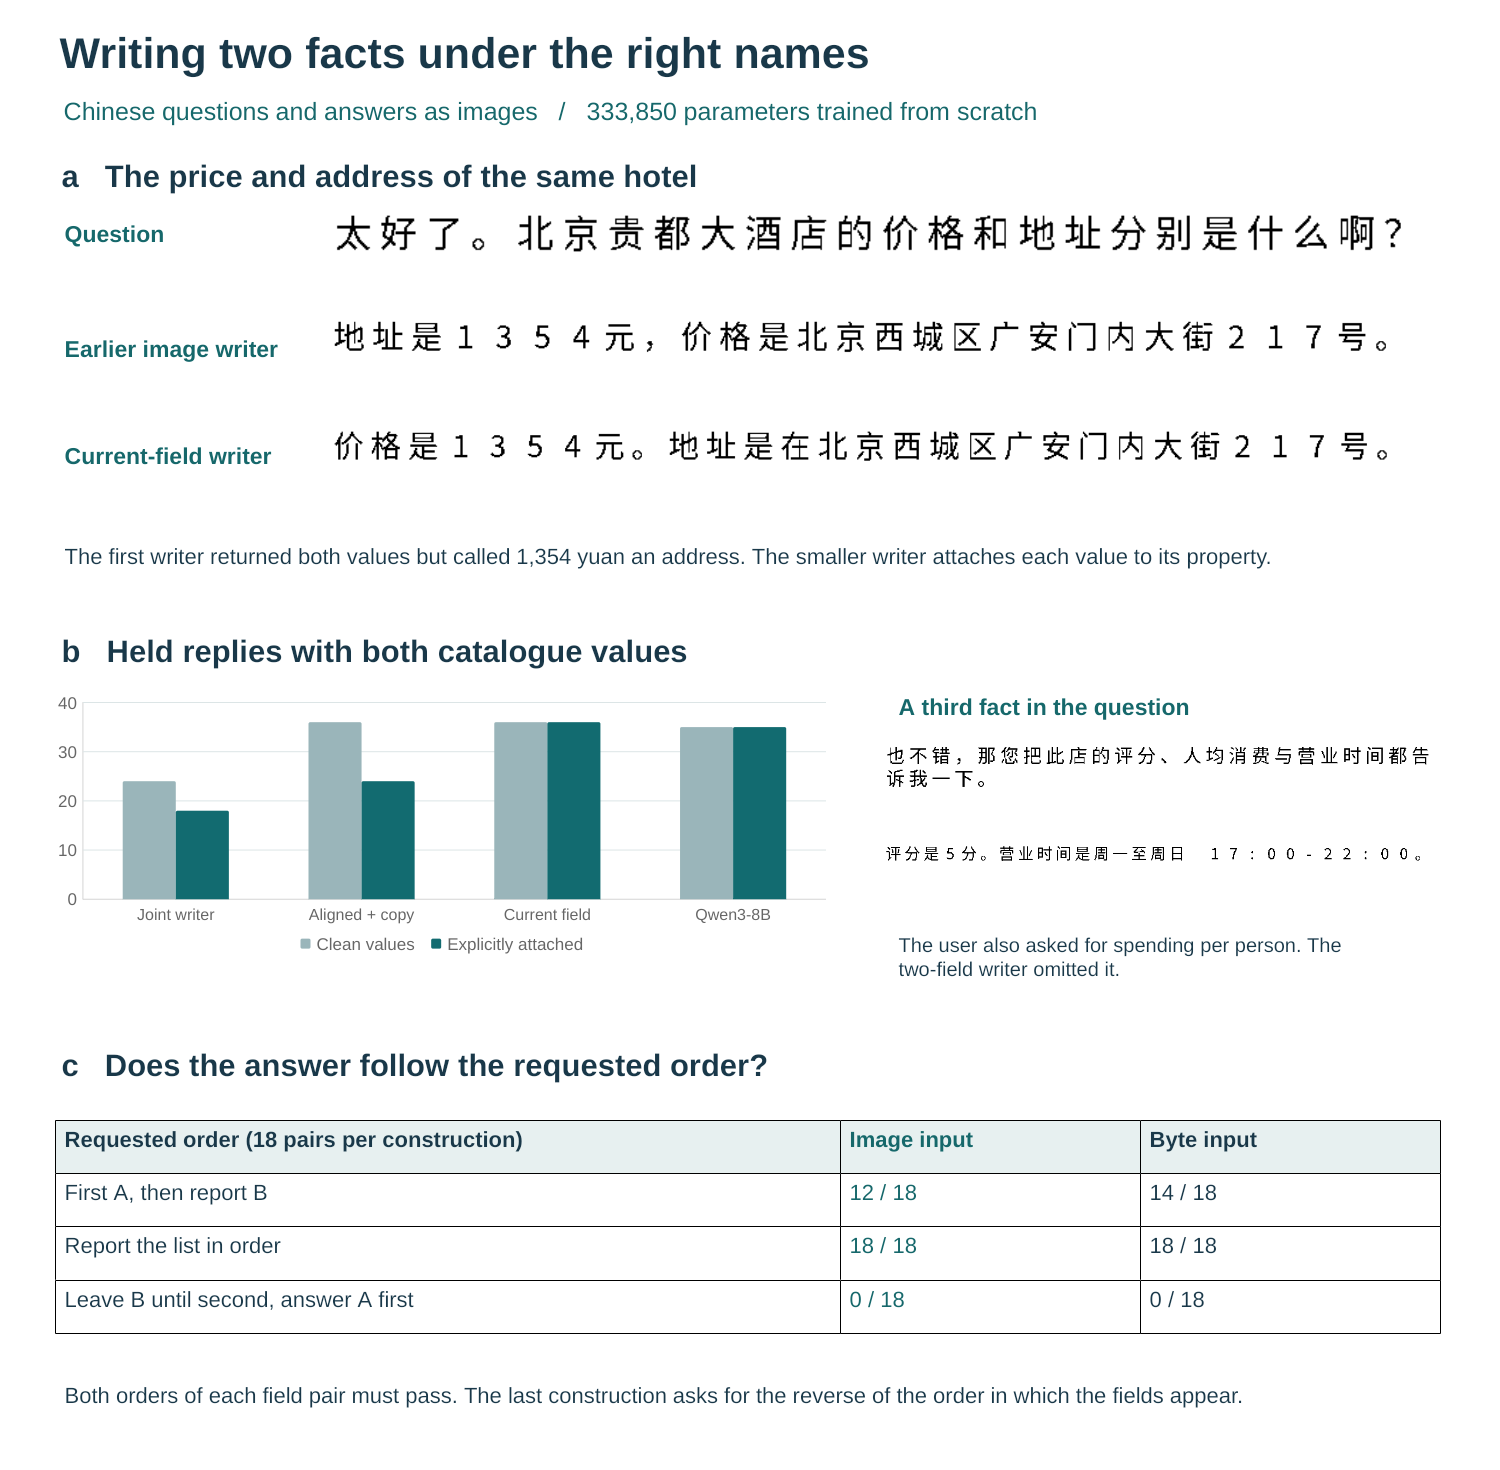
\includegraphics[width=.99\linewidth,height=.69\textheight,keepaspectratio]{../figures/Figure_141_two_fact_figure.png}
\end{center}
\small Panel a preserves actual output glyphs. In panel b the strict check requires each source value and an appropriate local field cue. It accepts 35 of 37 human references. Panel c tests three sentence constructions. Each row of eighteen pairs shares one construction. The last reverses the order of mention.\normalsize

\heading{Warm inference on one GPU}
Over 32 consecutive sweeps per measurement block, answering 37 questions took 0.393--0.492 seconds and 35.3--44.5 J per sweep for the compact writer. Two warm sweeps with local Qwen3-8B Q8 took 18.66--18.71 seconds and 4.17--4.23 kJ each. Both systems ran serially. The compact writer received prepared image cells and emitted copied spans and learned printed glyphs. Qwen received an ordinary text record over local HTTP. Preparation, loading and host energy are outside these measurements. The two systems have different scope.
\newpage
\heading{Figure 2. Questions, original output pixels and controls}
\begin{center}
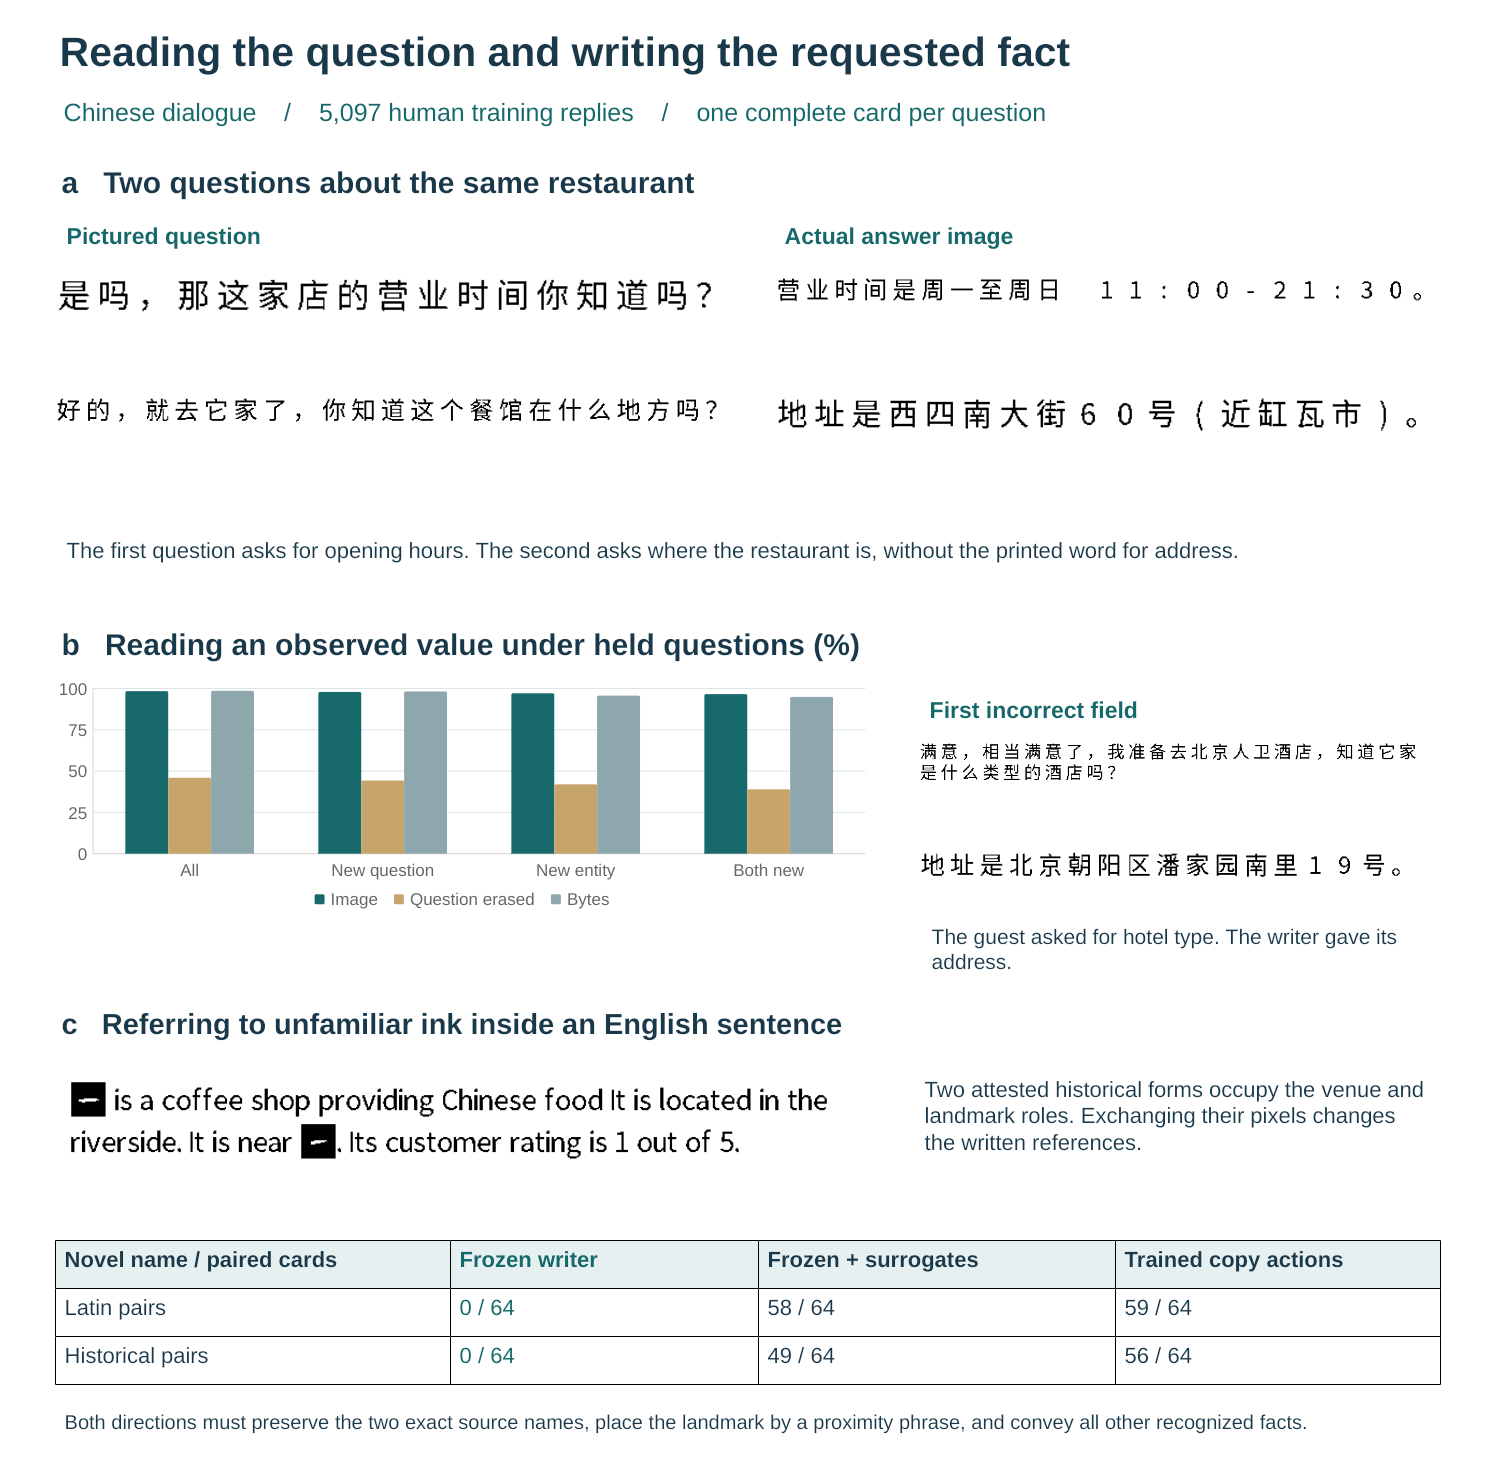
\includegraphics[width=.98\linewidth,height=.65\textheight,keepaspectratio]{../figures/Figure_140_visual_fact_reply.png}
\end{center}
\small Both Chinese inputs use the same venue record. The English sentence in panel c comes from a separate visual writer trained on human restaurant descriptions. Exchanging its pictured name and landmark preserved the original marks in all 128 novel-name pairs. Requiring both complete answers to carry the other facts reduced success to 59/64 Latin-name and 56/64 historical-mark pairs.\normalsize

\heading{Does word order matter?}
When two fields occurred in one question, the original reader got both directions right on nine of 54 controlled pairs. Replacing field names by identical pictured markers and learning which context denotes the request increased this to 54. On twelve further constructions, the new selector succeeded on ten and failed on two, compared with 58/216 complete pairs for the original reader and 180/216 after the change. None of the 515 natural questions activated the two-mention selector. Once the two field images are replaced by identical markers, swapping the field names leaves the visual context unchanged. For distinct fields, both answers have the correct role exactly when the selected position is correct. This is a checked Lean result. The eighteen swaps inside each frame share that positional decision.
\newpage
\heading{What changed when the meaning changed?}
The first eligible held record names Blue Spice, a pub serving Chinese food in the city centre, near Rainbow Vegetarian Caf\'e. The pictured policy excludes families. Figure~3 shows both returned pages after changing that single field. The writer changed sentence structure and polarity and kept the other facts. The candidates consisted of its own completions. The selector inferred the requested facts from the card.

The first card specified only a name, a coffee shop and the city centre. The writer added a high price. The final card named The Sorrento as the nearby landmark. The writer printed \emph{The Portel}. Both sentences are legible. Both would mislead a reader. In a source-visible, model-assisted assessment of twenty evenly spaced Chinese cards, the original greedy writer conveyed all facts without additions on 13 and the released system on 17. Several faithful sentences had awkward English. This reading has no independent human adjudication.

\heading{Dependence on the source}
The official test contains 1,847 fact combinations absent from training. Each selected English sentence differs from every full training reference under literal string comparison. After exchanging the test records cyclically, none of the selected Chinese-card outputs retained the exact requested literal fact set. Stock phrases and previously seen values remain available. \href{https://github.com/tuetschek/e2e-cleaning}{Cleaned E2E corpus and realization rules}.
\heading{Figure 3. What the writer actually printed}
\begin{center}
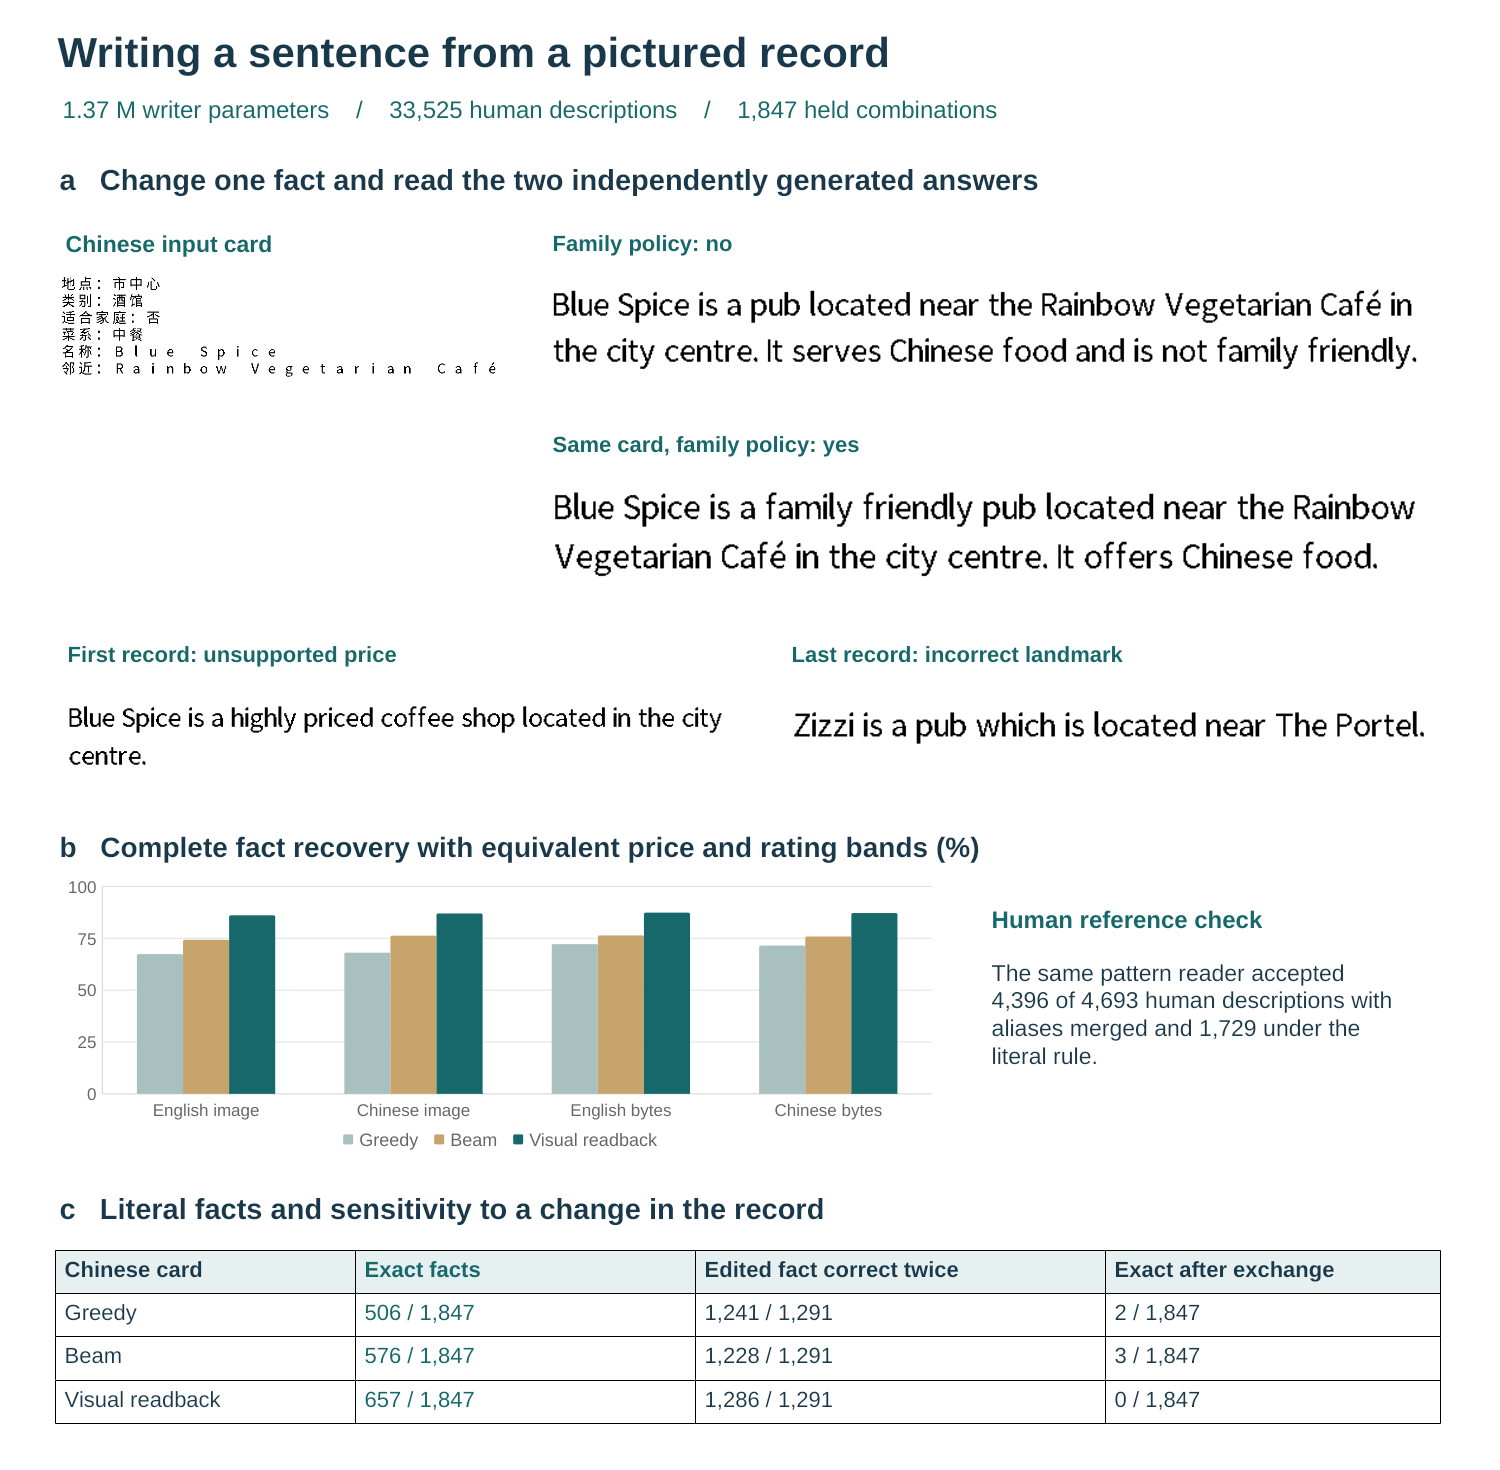
\includegraphics[width=.99\linewidth,height=.50\textheight,keepaspectratio]{../figures/Figure_139_semantic_page.png}
\end{center}
\small The original Chinese input and both answers preserve their physical glyph pixels. For display, blank sidebearings were trimmed and words were wrapped. The two errors are the first and last records in fixed test order. Each bar uses 1,847 unique meanings. The edited-fact column requires the requested family policy in the original answer and its opposite after the edit. Other factual errors can occur in the same pair.\normalsize
\newpage
\heading{How the visual writer learns}
English letters and Chinese characters use the same size cell. Their information content and linguistic functions can differ. The visual encoder maps a row of 32-pixel cells to a vector. Row order is randomized and row meaning is supervised during fitting. The decoder sees the set of row vectors and estimates
\[
 p(y\mid x)=\prod_{t=1}^{T+1} p(y_t\mid y_{<t}, E(x)),\qquad y_{T+1}=\mathrm{stop}.
\]
The writer uses a three-layer transformer across blocks of four glyphs. Within a block each cell can depend on earlier glyphs. Feedback comes from earlier emitted images. Choosing among 73 printable training bitmaps ensures sharp letters and restricts the alphabet. The optional Unicode transcript maps these particular bitmaps back to text.

\heading{Which error does reading back remove?}
The beam proposes eight stopped sentences. A 223,200-parameter inverse reader learned to recover facts from human descriptions presented as images. For a given card the selector uses its predicted field set, the writer's mean log likelihood and the inverse reader's Bernoulli log likelihood. Among $N$ cards let $C$ count those with a faithful candidate and $S$ those where the selected sentence is faithful. Then
\[
 N-S=(N-C)+(C-S).
\]
The merged-facts counts are $241=179+62$. The first 179 errors require better candidates. A perfect selector on this pool could recover at most 62 more. Enabling readback recovered 179 previously failed cases and lost 26 previously successful ones. The literal gains and losses were 71 and eight. A Lean proof gives a sufficient selection condition. If an ideal faithful witness exceeds every unfaithful score by more than twice the learned score's uniform error, a learned maximizer is faithful. The margin has yet to be established for these networks.

\heading{Controls and costs}
On a separately evaluated development set, interleaved Chinese and English rows gave 1,304 of 1,484 complete merged fact sets and 246 literal passes. The listener fit took 12.0 seconds and 1.49 kJ on one RTX 4090 D. Optical and byte writer fits took 113.0 and 115.2 seconds, consuming 11.51 and 11.72 kJ of device energy. The optical writer and listener have 1,591,210 parameters together. Host and cooling energy are excluded. Beam generation with readback for 3,138 Chinese cards consumed 4.66 kJ.

The scorer can mark both \emph{5 out of 5} and \emph{high} for one phrase. Merging such labels and corresponding price bands accepted 4,396 of 4,693 human references. Precision lost to merging and unrecognized invented facts limit this measure.
\newpage
\heading{Historical writing as evidence}
Some questions require a particular attested mark. A separate optical reader identified a headword and ordered fields in a pictured question about an illustrated dictionary. It returned their stored ink. One example below contains four historical exemplars. In another case unfamiliar wording led it to the wrong headword.
\begin{center}
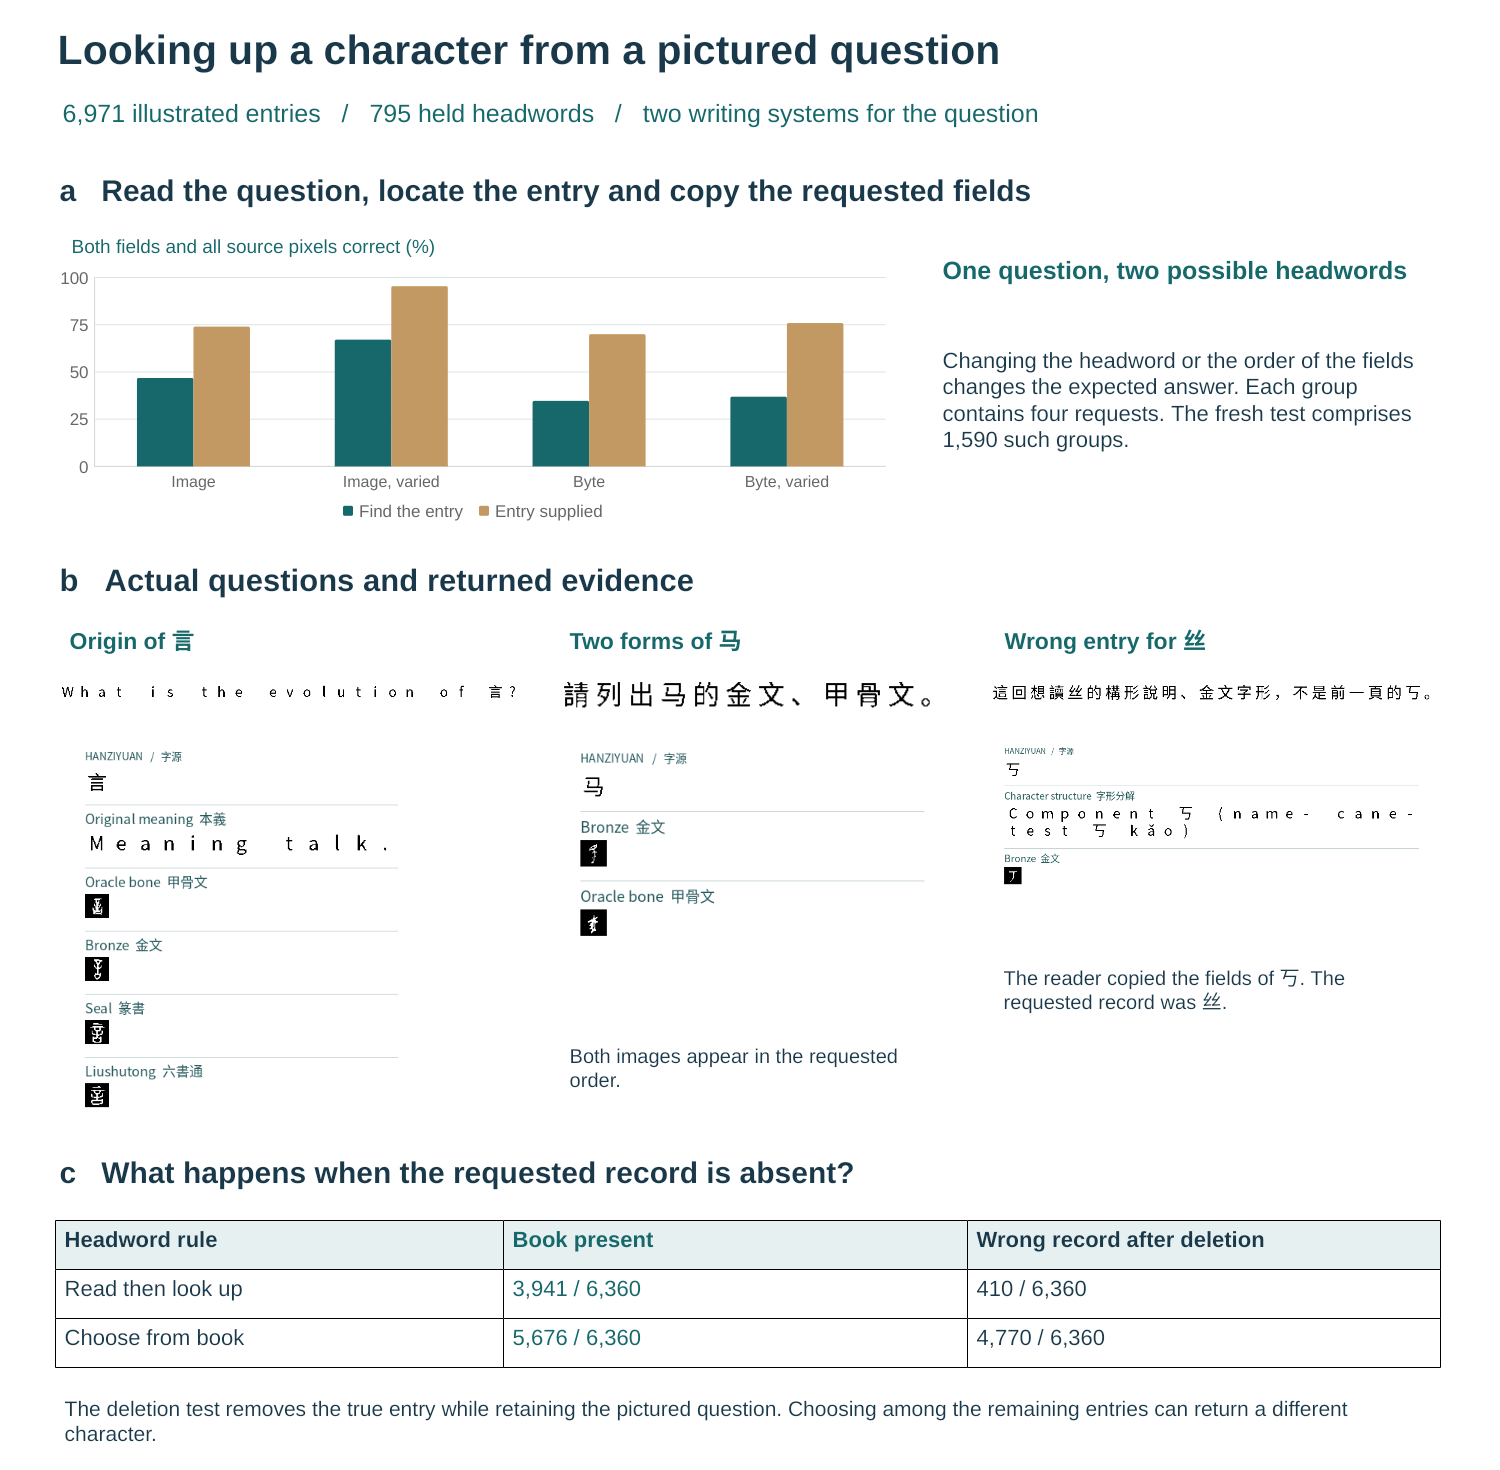
\includegraphics[width=.90\linewidth,height=.54\textheight,keepaspectratio]{../figures/Figure_138_glyph_atlas.png}
\end{center}
\small \textbf{Figure 4.} The experiment reused 795 held headword families across fresh wording. Field selection and page composition use a finite schema. Each form retains its source pixels. Inferring an unattested form needs different evidence.\normalsize

\heading{Relation to earlier work}
PIXAR demonstrated autoregressive text generation in pixel space. Earlier E2E systems used semantic reranking over generated text. Here the generator feeds back glyph images, the listener reads those images, and the byte reader shares the physical output task. Learning which evidence to use in an unlabelled paragraph requires a further transfer test. The current catalogue reader receives a resolved venue and visible field labels. \href{https://aclanthology.org/2024.findings-acl.874/}{Tai et al., 2024}. \href{https://ufal.mff.cuni.cz/~odusek/E2E/final_papers/E2E-ZHAW.pdf}{ZHAW E2E system}. \href{https://aclanthology.org/W17-5525/}{Novikova et al., 2017}.
\end{document}
